%%%%%%%%%%%%%%%%%%%%%%%%%%%%%%%%%%%%%%%%%
% University/School Laboratory Report
% LaTeX Template
% Version 3.1 (25/3/14)
%
% This template has been downloaded from:
% http://www.LaTeXTemplates.com
%
% Original author:
% Linux and Unix Users Group at Virginia Tech Wiki 
% (https://vtluug.org/wiki/Example_LaTeX_chem_lab_report)
%
% License:
% CC BY-NC-SA 3.0 (http://creativecommons.org/licenses/by-nc-sa/3.0/)
%
%%%%%%%%%%%%%%%%%%%%%%%%%%%%%%%%%%%%%%%%%

%----------------------------------------------------------------------------------------
%	PACKAGES AND DOCUMENT CONFIGURATIONS
%----------------------------------------------------------------------------------------

\documentclass{article}

\usepackage[version=3]{mhchem} % Package for chemical equation typesetting
\usepackage{siunitx} % Provides the \SI{}{} and \si{} command for typesetting SI units
\usepackage{graphicx} % Required for the inclusion of images
\usepackage{natbib} % Required to change bibliography style to APA
\usepackage{amsmath} % Required for some math elements 

\usepackage[utf8]{inputenc}
\usepackage[T1]{fontenc}

\setlength\parindent{0pt} % Removes all indentation from paragraphs
\setlength{\parskip}{1em}
\renewcommand{\labelenumi}{\alph{enumi}.} % Make numbering in the enumerate environment by letter rather than number (e.g. section 6)

%\usepackage{times} % Uncomment to use the Times New Roman font

%----------------------------------------------------------------------------------------
%	DOCUMENT INFORMATION
%----------------------------------------------------------------------------------------

\title{Laboration 3 \\ Design-Space Exploration with MPARM} % Title

\author{
  Björn \textsc{Hvass}\\
  Cyril \textsc{Barrelet}
} % Authors name

\date{\today} % Date for the report

\begin{document}

\maketitle % Insert the title, author and date

\begin{center}
\begin{tabular}{l r}
Course: & TDTS07\\ % Date the experiment was performed
Liu Ids: & Hvass bjohv276\\ % Partner names
& Barrelet cyrba593 \\
\end{tabular}
\end{center}

% If you wish to include an abstract, uncomment the lines below
% \begin{abstract}
% Abstract text
% \end{abstract}

\newpage\section{Design-Space Exploration for Energy Minimization}

In this section, different parameters are tested, like the frequency and the cache size, to find the greatest parameter to minimaze the energy consumption. 

Here is the test table:

\begin{table}[]
\begin{tabular}{lllllll}
Test & Frequency (mHz) & Divider & Energy spent (μJ) & Execution time (ms) & Cache size (bytes) & Cache type        \\
1    & 200             & 1       & 45.03             & 3.42                & 4096               & Fully associative \\
2    & 100             & 2       & 34.37             & 3.42                & 4096               & Fully associative \\
3    & 67              & 3       & 33.53             & 4.99                & 4096               & Fully associative \\
4    & 50              & 4       & 33.43             & 6.35                & 4096               & Fully associative \\
5    & 25              & 8       & 33.35             & 12.39               & 4096               & Fully associative \\
6    & 200             & 1       & 45.64             & 1.69                & 8192               & Fully associative \\
7    & 100             & 2       & 34.97             & 3.42                & 8192               & Fully associative \\
8    & 200             & 1       & 44.76             & 1.69                & 2048               & Fully associative \\
9    & 100             & 2       & 34.09             & 3.42                & 2048               & Fully associative
\end{tabular}
\end{table}

As regarding energy consumption, the cache size has a low impact on the energy consumption for the same frequency.
In the second hand, when the divider is set to decrease the frequency, the power consumption decrease as well to tend to be around 33.5 μJ. However, the execution time is also increased. 

The greatest parameters set according to the test table to find the best energy consumption and the best execution time is to set the divider as 2 and the cache size as 2048 bytes.
\newpage\section{Assignment 2}
Efficiency comparison of shared memory and distributed message passing.  To gather the results presented below, see the table below, two different GSM voice codec implementations was used and simulated in mparm. Using mparm some tests were conducted to asses the impact that the frequency of the different processors had upon the system.  By reducing the frequency with a divider of 2 as can be seen in test 6 in the table, both the traffic and the busyness of the bus has been reduced quite a lot.  Compared to the first test where the system ran with the default settings this is an improvement of efficiency and energy consumption without sacrificing to much execution time.

\begin{table}[]
\begin{tabular}{lllllll}
  & \begin{tabular}[c]{@{}l@{}}Frequency (MHz)\\ p0 | p1 | p2\end{tabular} & Communication & Bus busy (\% of master cycles) & Bus transferring (\% of master cycles) & Energy spent (μJ) & Exec time (ms) \\
1 & 200 | 200 | 200                                                        & Queue         & 56.25                          & 20.63                                  & 605               & 10             \\
2 & 200 | 200 | 200                                                        & Shared        & 44.91                          & 17.2                                   & 895               & 14             \\
3 & 100 | 200 | 200                                                        & Shared        & 37.39                          & 13.31                                  & 910               & 18.85          \\
4 & 200 | 100 | 200                                                        & Shared        & 39.43                          & 14.22                                  & 769               & 14.09          \\
5 & 200 | 200 | 100                                                        & Shared        & 36.61                          & 13                                     & 999               & 21.5           \\
6 & 100 | 100 | 100                                                        & Shared        & 23.57                          & 8.25                                   & 589               & 26.23          \\
7 & 67 | 67 | 67                                                           & Shared        & 16.54                          & 5.77                                   & 578               & 37.6           \\
8 & 67 | 100 | 100                                                         & Shared        & 20.39                          & 7.13                                   & 614               & 31.5          
\end{tabular}
\end{table}

\newpage\section{Mapping/Scheduling Exercice}

This exercise talks about improving the execution time of an application by changing the Scheduling and the Mapping of the tasks.

\subsection{New schedule}

As regarding the data dependencies, this schedule has been created to have the minimal length.

\bigskip

\begin{figure}[h!]
  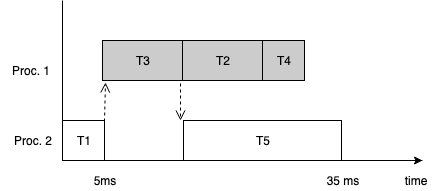
\includegraphics[width=\textwidth]{Ass3_1.png}
  \caption{New schedule}
  \label{fig:sys}
\end{figure}

By changing the schedule without changing the mapping, the goal is to find the best scheduling to avoid the wast of time.
The task T3 is required to allow the execution of T5 which is the longest task. T5 doesn't require T2 and T4, so T3 has to be before T2 to avoid that waste of time.

\newpage\subsection{New mapping}

This new schedule has been constructed by changing the mapping of tasks to processors. 

\bigskip

\begin{figure}[h!]
  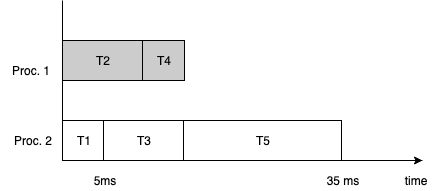
\includegraphics[width=\textwidth]{Ass3_2.png}
  \caption{New mapping}
  \label{fig:sys}
\end{figure}


By changing the mapping, the goal is to condense the tasks as much as possible. 
The tasks T1, T3, and T5 are dependent on each other and they need to be ordered like that. So a single processor can handle those different tasks. 
In the second hand, the tasks T2 and T4 can be run by another processor at the same time as T1, T2, and T5.



%----------------------------------------------------------------------------------------


\end{document}
